\section{Theory}\label{sec:Theory}

\newcommand{\state}{\ket{\psi}}
\newcommand{\hoket}{\ket{\phi}}
\newcommand{\hoep}{\ket{\phi +}}
\newcommand{\hoem}{\ket{\phi -}}
\newcommand{\pin}{\psi_\text{in}}
\newcommand{\pout}{\psi_\text{out}}
\newcommand{\kpin}{\ket{\psi_\text{in}}}
\newcommand{\kpout}{\ket{\psi_\text{out}}}
\newcommand{\mop}{\Omega_{+}}
\newcommand{\mom}{\Omega_{-}}
\newcommand{\melt}[3]{\left|\mel{#1}{#2}{#3}\right|^{2}}
\newcommand{\scat}{\mathcal{S}}
\newcommand{\mscat}{\(\scat\)}
\newcommand{\oop}[1]{\mathcal{#1}}
\newcommand{\moop}[1]{\(\oop{#1}\)}
Quantum scattering is a very complicated process, behaving so differently from the
classical case of billiard balls that our intuition breaks down. Fortunately, the intricacies of
the scattering process itself can be conveniently omitted by instead focusing on
the relationship between the initial and resulting states, illustrated in FIGURE.
Specifically, the true state \(\ket{\psi}\) is related to the asymptotic
incoming and outgoing states \(\kpin\) and \(\kpout\) through the so-called
\textit{M\o ller operators} \(\Omega_{\pm}\):

\begin{align*}
  \state &= \mop\kpin = \hoep\\
  \state &= \mom\kpout = \hoem .
\end{align*}
[Add some history of Møller]

If time dependence is added, the M\o{}ller operations allows one to move between
the asymptotic states and the actual state at time \(t\).
Combining them, the outgoing state is related to the incoming state by

\begin{equation*}
  \kpout = \mom^{\dagger}\mop\kpin = \scat\kpin
\end{equation*}

giving the definition of the \textit{scattering operator} \mscat.
In the general case let \(\ket{\chi -}\) and \(\ket{\Phi +}\) by any arbitrary
orbits. The probability of the process \(\ket{\chi -}\leftarrow\ket{\Phi +}\)
occurring is
then the square of the  matrix element of\ \mscat :

\begin{equation*}
  w(\chi \leftarrow \Phi) = \left| \ip{\chi -}{\Phi +} \right|^{2} = \melt{\chi}{\scat}{\Phi}.
\end{equation*}

The probability \(w\) is itself not observable, however, the related quantity
cross-section \mbox{\(\sigma(\chi \leftarrow \Phi)\)} is. The outgoing particle can
scatter in a solid angle \(d\Omega\), oriented in the direction of momentum
\(\vec{p}\). Likewise, the incoming particle can be described as wave packets
with narrowly defined momentum \(\vec{p_{0}}\). It can then be shown that[CITE] the
differential cross section is

\begin{align*}
  \dv{\sigma}{\Omega}(\vec{p}\leftarrow\vec{p_{0}}) = \left| f(\vec{p}\leftarrow\vec{p_{0}}) \right|^{2}
\end{align*}
with \(f(\vec{p}\leftarrow \vec{p_{0}})\) being the scattering amplitude, as known from elementary scattering
theory. Note that only the magnitude of \(f\) can be obtained through the
cross-section.

The next step is to relate cross-section to the scattering operator. It
can be shown that \mscat{} commutes with the free Hamiltonian\( \oop{H}_{0}\)
\begin{align*}
  \oop{H} = \oop{H}_{0} + V &\qquad [\oop{H}_{0}, \scat{}] = 0
\end{align*}
Letting \(\ket{\vb{p}}\) be the eigenvectors of \(\oop{H}_{0}\) in momentum
basis, we have
\begin{align*}
  \mel{\vb{p}^{\prime}}{[\oop{H}_{0}, \scat]}{\vb{p}} = (E_{p^{\prime}}-E_{p})\mel{\vb{p}^{\prime}}{\scat}{\vb{p}} = 0
\end{align*}
implying that \(\mel{\vb{p}^{\prime}}{\scat}{\vb{p}}\) is zero except for
\(E_{p^{\prime}}=E_{p}\). This leads to the form
\begin{align*}
  \mel{\vb{p}^{\prime}}{\scat}{\vb{p}} = \delta(E_{p^{\prime}}-E_{p})\times\text{remainder}
\end{align*}

At this point it is fruitful to define a new operator \(\oop{R} \equiv 1 -
\scat\). \moop{R} is the difference between the case of scattering and no scattering. It too commutes with \(\oop{H}_{0}\), and so has the form
\begin{align*}
  \mel{\vb{p}^{\prime}}{\oop{R}}{\vb{p}} = -2\pi i\delta(E_{p^{\prime}}-E_{p})t(\vb{p}^{\prime}\leftarrow \vb{p})
\end{align*}
with the factors \(-2\pi i\) and \(t(\vb{p}^{\prime}\leftarrow\vb{p})\)
introduced for future convenience. The elements of\ \mscat{} can therefore be written 
\begin{align*}
  \mel{\vb{p}^{\prime}}{\scat}{\vb{p}} = \delta(\vb{p}^{\prime} - \vb{p}) - 2\pi i \delta(E_{p^{\prime}}-E_{p})t(\vb{p}^{\prime}\leftarrow \vb{p}).
\end{align*}
The first term describes the situation where no scattering occurs, while the
second is the amplitude when the wave is actually scattered. The function
\(t(\vb{p}^{\prime}\leftarrow \vb{p})\) is continuous for most potentials and
analytic for many, but only defined for the ``shell'' \(\vb{p}^{{\prime}^{2}} =
\vb{p}^{2}\). However unphysical, it is computationally beneficial to define an
operator \moop{T} whose matrix elements \(\mel{\vb{p}^{\prime}}{T}{\vb{p}}\) are defined for all \(\vb{p}\) and
coincide with the values of \(t\) on the shell.

The scattering amplitude can be shown to be related to the on-shell \moop{T}
matrix elements as[cite]
\begin{align*}
  f(\vb{p}^{\prime} \leftarrow \vb{p})= -(2\pi)^{2}mt(\vb{p}^{\prime}\leftarrow\vb{p}).
\end{align*}
The elements of the scattering matrix can from this be directly related to the
scattering amplitude as
\begin{align*}
  \mel{\vb{p}^{\prime}}{\scat}{\vb{p}} = \delta(\vb{p}^{\prime} - \vb{p}) - \frac{i}{2\pi m}\delta(E_{p^{\prime}}-E_{p})f(\vb{p}^{\prime}\leftarrow \vb{p}).
\end{align*}

\subsection{Spherical Coordinates}

Introducti

As known from elementary quantum mechanics, \(\oop{H}^{0}\) commutes with the
angular momentum operator \(\oop{L}^{2}\) and z-axis projection \(\oop{L}_{3}\).
These three operators form a complete set of commuting observables. Since
\mscat{} commutes with \(\oop{H}^{0}\), \mscat{} too commutes with the
aforementioned 
operators, and is diagonal in the common basis, namely the basis of spherical waves
\(\left\{ \ket{Elm} \right\}\), with \(E, l(l+1)\) and \(m\) being the
eigenvalues for \(\oop{H}^{0}\),  \(\oop{L}^{2}\) and  \(\oop{L}_{3}\)
respectively. Since this basis diagonalizes\ \mscat{}, its matrix elements are
\begin{align*}
  \mel{E^{\prime}l^{\prime}m^{\prime}}{\scat}{Elm} = \delta(E^{\prime}-E)\delta_{l^{\prime}l}\delta_{m^{\prime}m}s_{l}(E).
\end{align*}

\mscat{} can be shown to be unitary, implying the eigenvalues \(s_{l}(E)\) must have
modulus one, justifying the form
\begin{align*}
  \mel{E^{\prime}l^{\prime}m^{\prime}}{\scat}{Elm} = \delta(E^{\prime}-E)\delta_{l^{\prime}l}\delta_{m^{\prime}m}\exp(2i\delta_{l}(E))
\end{align*}
The quantity \(\delta_{l}(E)\) is the important \textit{phase shift}, an
observable obtainable from both experiment and numerical calculations. It is
purely real with an inherent ambiguity modulo \(\pi\), as seen from
\begin{align*}
  \exp(2i[\delta_{l}+n\pi]) = \exp(2i\delta_{l})\exp(2in\pi) = \exp(2i\delta_{l}).
\end{align*}

[Meaning of T in the sense incident plane wave]
[]

The decomposition of \(f(\vb{p}^{\prime}\leftarrow\vb{p})\) into partial waves
can be obtained by exploiting the relation

\begin{equation}
  \label{eq:sp1}
  \mel{\vb{p}^{\prime}}{(\scat-1)}{\vb{p}} = \frac{i}{2\pi m}\delta(E^{\prime}-E)f(\vb{p}^{\prime}\leftarrow \vb{p}).
\end{equation}
Inserting a complete set of states of the left hand side gives
\begin{align*}
  \mel{\vb{p}^{\prime}}{(\scat-1)}{\vb{p}} &= \int \dd E \sum_{l, m}  \mel{\vb{p}^{\prime}}{(\scat-1)}{Elm}\ip{Elm}{\vb{p}}\\
                                             &=  \int \dd E \sum_{l, m} (s_{l}(E)-1) \ip{\vb{p}^{\prime}}{Elm}\ip{Elm}{\vb{p}}\\
  &= \frac{1}{mp}\delta(E_{p^{\prime}}-E_{p})\sum_{l,m}Y_{l}^{m}(\vu{p}^{\prime})[s_{l}(E_{p})-1]Y^{m}_{l}(\vu{p})^{*}
\end{align*}
where \(Y_{l}^{m}\) is the spherical harmonical and hat denotes unit vector. Combining this
with~\eqref{eq:sp1}, the amplitude can be decomposed to

\begin{align*}
  f(\vb{p}^{\prime}\leftarrow\vb{p}) = \frac{2\pi}{ip}\sum_{l,m}Y_{l}^{m}(\vu{p}^{\prime})[s_{l}(E_{p})-1]Y^{m}_{l}(\vu{p})^{*}
\end{align*}
Letting \(\vu{p}\) lie along \(z\) and noting independence of \(m\) [WHY], we
define
\begin{align*}
  f(E_{p},\theta) \equiv f(\vb{p}^{\prime}\leftarrow\vb{p})=\frac{1}{2ip}\sum_{l}(2l+1)[s_{l}(E_{p})-1]P_{l}(\cos\theta)
\end{align*}
This leads to the natural definition of the \textit{partial wave amplitude} as
\begin{align*}
  f_{l}(E) \equiv \frac{s_{l}(E)-1}{2ip} = \frac{\exp[ 2i\delta_{l}(\theta)] - 1}{2ip} = \frac{\exp[2i\delta_{l}(E)]\sin\delta_{l}(E)}{p}
\end{align*}
Analogously the total cross-section can be decomposed into \textit{partial wave
  cross-sections}, giving
\begin{align*}
  \sigma(p) = \sum_{l}\sigma_{l}(p) = \sum_{l}4\pi(2l+1)\left| f_{l}(p) \right|^{2} = \sum_{l}4\pi(2l+1)\frac{\sin^{2}\delta_{l}}{p^{2}}
\end{align*}
The magnitude of each partial wave cross-section is from this constrained by the
so called \textit{unitary bound}: 
\begin{align*}
  |\sigma_{l}| \leq 4\pi\frac{2l+1}{p^{2}}.
\end{align*}
The maximal value is only reached if
\(\delta_{l}\) is an odd multiple of \(\pi/2\)

\subsection{Green's Function}
One of the most important tools in scattering theory is \textit{the resolvent},
or \textit{Green's operator}. For many types of integral equations, a Green's
function can be associated, transforming the solving of the equation to the
computation of the Green's function. For our purposes the most important Green's
operators are the \textit{free Green's operator}

\begin{equation*}
  \oop{G}^{0}(z) \equiv (z-\oop{H}^{0})^{-1}
\end{equation*}
and the \textit{full Green's operator}
\begin{equation*}
  \oop{G}(z) \equiv (z-\oop{H})^{-1}
\end{equation*}
with \(z\in\mathbb{C}\). Without loss of generality, assume the spectrum of
\(\oop{H}\) is discrete, with the orthonormal basis \({\ket{n}}\). Then the full
Green's operator can be written

\begin{equation*}
  \oop{G}(z) = (z-\oop{H})^{-1}1 = \sum_{n}\frac{\op{n}}{z-E_{n}}.
\end{equation*}
A specific matrix element is therefore
\begin{equation*}
  \mel{\chi}{\oop{G}(z)}{\psi} =\sum_{n} \frac{\ip{\chi}{n}\ip{n}{\psi}}{z-E_{n}}.
\end{equation*}
\newcommand{\gop}{\oop{G}(z)}
\newcommand{\mgop}{\(\oop{G}(z)\)}
For any \(z\) not an eigenvalue \(E_{n}\), the matrix element is well defined and
analytic. When \(z\) is an eigenvalue, it is a simple pole with residue
\(\ip{\chi}{n}\ip{n}{\psi}\). That is, knowing the poles of \(\oop{G}(z)\) gives
information about the corresponding eigenvectors. As both the energy
eigenvectors and eigenvalues can be found from \mgop{} itself, knowledge of
\mgop{} is equivalent to solving the eigenvalue problem of
\(\oop{H}\)\footnote{Of course, this is merely an intuitive explanation, not a
  proof. It can be shown that this is indeed true in the general case.}.

While discrete spectra lead to poles in \(\mel{\chi}{\gop{}}{\psi}\), continuous spectra lead to 
branch cuts. Consider the free Green's operator, which in terms of the angular
momentum eigenvectors in analogy to the discrete spectrum has the matrix elements

\begin{equation*}
  \mel{\chi}{\oop{G}^{0}(z)}{\psi} = \int_{0}^{\infty}\frac{\dd E}{z-E}\left\{
  \sum_{l,m}\ip{\chi}{Elm}\ip{Elm}{\psi}
  \right\}
\end{equation*}

which again gives well-defined functions for \(z\notin\mathbb{R}^{+}\). For any
\(E^{0} > 0\), the integral diverges. This can be seen by taking the difference
between approaching the axis from the top and approaching it from the bottom,
which can be shown to yield \(2\pi i \sum_{lm}\op{Elm}\).

The scattering process can yield both scattered states and bound states. The
former is associated with continuous spectra while the latter with discrete.
From the discussion above, scattered states are associated with branch cuts
along \(E^{0}>0\) while bound states show up as simple poles in \(\oop{G}(z)\).

Finding \(\oop{G}(z)\) is just as difficult as solving the eigenvalue problem
for \(\oop{H}\). Using \(\oop{G}(z)\), however, yields an alternative numerical
approach while at the same providing a powerful theoretical tool. The first step
is to write \(\oop{G}(z)\) in terms of the simpler \(\oop{G}^{0}(z)\). This is
trivially done using the algebraic relation

\begin{equation*}
  \oop{A}^{-1} = \oop{B}^{-1} + \oop{B}^{-1}(\oop{B}-\oop{A})\oop{A}^{-1}.
\end{equation*}
Inserting \(\oop{A} = z-\oop{H}\) and \(\oop{B} = z-\oop{H}^{0}\) gives
\begin{equation}
  \label{eq:LSG}
  \gop = \gop{}^{0} + \gop{}^{0}V\gop{} = \gop{}^{0} + \gop{}V\gop{}^{0}.
\end{equation}
This is known as the \textit{Lippmann-Schwinger equation for \mgop{}}.


\subsection{Lippman Schwinger}

The Lippmann-Schwinger equation turns out to be a common and useful relation
between operators in scattering theory. The derivation through Green's operators
is not the historic path, and has the downside of obscuring its physical
relationship to the Schr\"odinger equation.
[Mer historie]

[intro]
Out of thin air we define the operator \(\oop{T}\) as the potential plus the
distortion to the potential caused by the full Green's operator:

\begin{equation}
  \label{eq:T}
  \oop{T}(z) = V + V\oop{G}V.
\end{equation}
It is clear that \(\oop{T}(z)\) has the same properties as \mgop{} with respect
to poles and branch cuts. Combining~\eqref{eq:T} with~\eqref{eq:LSG} together
with some algebraic manipulations, we obtain the Lippmann-Schwinger equation for \(\oop{T}(z)\):

\begin{equation}
  \label{eq:LST}
 \oop{T}(z) = V + V\oop{G}^{0}(z)\oop{T}(z).
\end{equation}

In momentum space~\eqref{eq:LST} is written as

\begin{equation*}
  \mel{\vb{p}^{\prime}}{\oop{T}(z)}{\vb{p}} = \mel{\vb{p}^{\prime}}{V}{\vb{p}}
  + \int\dd^{3}p^{''} \frac{\mel{\vb{p}}{V}{\vb{p^{''}}}}{z-E_{p^{''}}}\mel{\vb{p}^{''}}{T(z)}{\vb{p}}
\end{equation*}

This highlights the need for introducing the \(\oop{T}\) operator in the first
place. There is no LS equation for the \(\oop{S}\) because it requires the
operators to be smooth functions, while \(\oop{S}(z)\) is
highly singular. On the other hand \(\oop{T}\) analytic almost everywhere,
allowing it to be expressed in terms of an integral equation. 

Through a long and rather limit-finicky derivation, the \moop{S} operator can be
derived in terms of the \moop{T} operator when \(z\) approaches the real axis
from above
\begin{equation*}
  \mel{\vb{p}\prime}{S}{\vb{p}} = \delta(\vb{p}^{\prime}-\vb{p}) -2\pi i\delta(E_{p^{\prime}}-E_{p})
  \lim_{\epsilon\downarrow 0}\mel{\vb{p}^{\prime}}{T(E_{p}+i\epsilon)}{\vb{p}}.
\end{equation*}
This relation being the main motivation for defining \moop{T} in the first
place. It shows that \(t(\vb{p}^{\prime}\leftarrow\vb{p})\) corresponds to the
on-shell \(T\)-matrix.

A reasonable question to ask is why computing the entire \(T\)-matrix is
necessary when only the on-shell elements are physical. As already mentioned,
one reason is computational; The on-shell elements are the limiting quantities
of the off-shell elements. This doesn't mean that the off-shell elements are
only a mathematical necessity. In fact, they correspond to the virtual
interactions in the scattering process, which accounts for their fundamental
unmeasurable nature. We are only allowed to observe the scattering in the
non-interacting region, being the limiting case of the unobservable processes
happening inside of the interacting region. Our initial starting point of
focusing on the asymptotic states while ignoring the intricacies of the
scattering is therefore not some mathematical trick to make computation easier,
but an unavoidable requirement.

\subsection{The K-Matrix}

The Lippmann-Schwinger equation for \(\oop{T}\) can not be solved by simple
analytical methods. One recourse is to use approximation techniques. These are
based on the expansion of \(\oop{T}\) into the 
infinite sum
\begin{equation*}
  \oop{T} = V + V \frac{1}{E-H^{0}+i\epsilon}V + V \frac{1}{E-H^{0}+i\epsilon}V \frac{1}{E-H^{0}+i\epsilon} V+\ldots
\end{equation*}
The unitarity condition of \(\oop{T}\) is satisfied for the whole series, but
violated for any finite order. If the series happens to be rapidly convergent,
it may not pose a problem for numerical methods\footnote{That is to say, if the
  process described is sufficiently inelastic, energy will be approximately
  conserved.~\cite{Le_Ru_2013}}. Nevertheless, a more stable
approach is to enforce unitarity. The Caley 
transform achieves this, whereby a operator is constructed in such a way as to
ensure unitary.

The Caley transform of \(\oop{S}\) is denoted by \(\oop{M}\), and is defined
as

\begin{equation*}
  \oop{M} = i \frac{1-\oop{S}}{1+\oop{S}}.
\end{equation*}
The \(K\)-matrix\footnote{The nomenclature of the \(K\)-matrix is a mess. It is
  also called the \(R\)-matrix, the \(T\)-matrix, the reaction matrix, the
  reactance matrix, the dampening matrix, the distortion matrix, the dissipative
  matrix, and Heitler's
  matrix. To avoid overworking any of the other
  letters, I follow the style of Taylor.} is the matrix elements of the\
\moop{M} operator:
\begin{equation*}
  \mel{\vb{p}^{\prime}}{\oop{M}}{\vb{p}} = \delta(E_{p^{\prime}}-E_{p})k(\vb{p}^{\prime}\leftarrow\vb{p}).
\end{equation*}

When\ \moop{S} is symmetric,\ \moop{M} is both Hermitian and
symmetric, implying its matrix elements are real.
As with\ \moop{S} and\ \moop{R}, \moop{M} becomes diagonal in the basis
\(\left\{ \ket{Elm} \right\}\):
\begin{align*}
  \mel{E^{\prime}l^{\prime}m^{\prime}}{\oop{S}}{Elm} &= \delta(E_{p^{\prime}}-E_{p})\delta_{l^{\prime},l}\delta_{m^{\prime},m}s_{l}(E)\\
  \mel{E^{\prime}l^{\prime}m^{\prime}}{\oop{R}}{Elm} &= \delta(E_{p^{\prime}}-E_{p})\delta_{l^{\prime},l}\delta_{m^{\prime},m}2ipf_{l}(E)\\
  \mel{E^{\prime}l^{\prime}m^{\prime}}{\oop{M}}{Elm} &= \delta(E_{p^{\prime}}-E_{p})\delta_{l^{\prime},l}\delta_{m^{\prime},m}k_{l}(E).\\
\end{align*}
The elements \(k_{l}(E)\) will in this case be real, and are directly related to
the phase shifts:
\begin{align*}
  k_{l} = i \frac{1-s_{l}}{1+s_{l}} = \tan\delta_{l}.
\end{align*}

[fix factor 1/p]

%The \(K\)-matrix is to\ \moop{M} as \(T\) is to\ \moop{R}.
It can be shown that in the same way as\ \moop{S} is related to expansion into
plane wave stationary states \(\ket{\vb{p}\pm}\),\ \moop{M} is related to expansion into standing
waves \(\ket{\vb{p}s}\)

[Expand a bit on standing waves]

[Derive Heitler's equation]
\subsection{Bound States and Levinson's Theorem}
[The Jost function]
[Poles of S]
[Levinson]

\subsection{Potentials}
\subsubsection{The Square Well}
Near and dear to everyone is the square well potential; a simple discontinuous
potential with value \(V\_{0}\) in the interacting region and zero everywhere
else:
\begin{equation*}
  V(r) =
  \begin{cases}
    V_{0} & \text{for } 0 \leq r \leq R\\
    0 & \text{for } r > R 
  \end{cases}
\end{equation*}

The potential is plotted in~\cref{fig:squarewell}

\begin{figure}[H]
  \centering
  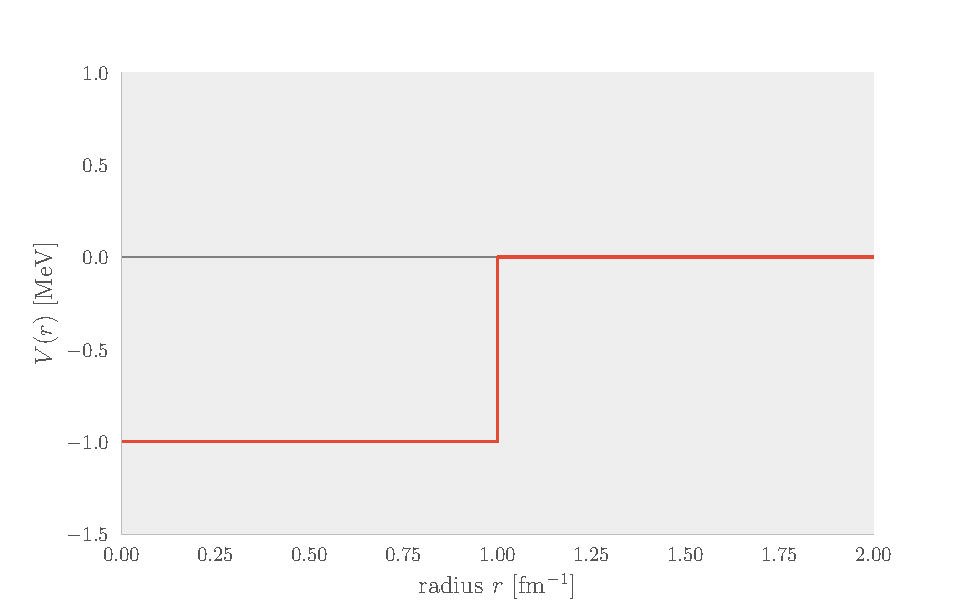
\includegraphics[]{Figures/squarewell.pdf}
  \caption{\label{fig:squarewell} An attractive square well potential with
    \(V_{0}=-1\) MeV.}
\end{figure}

[Analytical Solutions]


\subsubsection{The Yukawa Potential}
[HISTORY]

The Yukawa potential was later generalized into a class of \textit{generalized
  Yukawa potentials}. They are potentials build on superpositions of Yukawa potentials:
\begin{equation*}
  V(r) = \sum_{i=1}^{N}C_{i}\frac{e^{-\eta_{i}r}}{r}
\end{equation*}
for some coefficients \(C_{i}\) and \(\eta_{i}\).

A specific instance of a generalized Yukawa potential is the \textit{Reid potential}. It
is a parameterized potential between a proton and a neutron for the partial wave
\(^{1}S_{0}\), consisting of three terms:
\begin{equation*}
  V(r) = V_{a}\frac{e^{-ax}}{x} + V_{b}\frac{e^{-bx}}{x} + V_{c}\frac{e^{-cx}}{x}
\end{equation*}
where \(x=\mu r\), \(\mu=0.7\) MeV, \(V_{a}=-10.463\) MeV, \(V_{b}=-1650.6\)
MeV, \(V_{c}=6484.3\) MeV, and \(a=1\), \(b=4\) and \(c=7\).
[History of Reid].

\subsubsection{Momentum Basis}

Going from position basis to momentum space requires a change of basis, achieved
through a Fourier transform. The problem is multidimensional, requiring a
generalized Fourier transform. As we are only dealing with spherically symmetric
and central potentials, the more suitable Hankel transform\footnote{The Hankel
  transform can be regarded as the Fourier transform in hyperspherical coordinates, expanding the function in
Bessel functions instead of sines and cosines. } can be used. For
\(s\)-waves, it takes the form:

\newcommand{\kp}{k^{\prime}}
\begin{equation*}
  V_{l}(k, \kp{}) = \int_{0}^{\infty}j_{0}(kr)V(r)j_{0}(k^{\prime}r)r^{2}\dd r .
\end{equation*}


[Square well in momentum basis]

[Reid in momentum basis]




%%% Local Variables:
%%% mode: latex
%%% TeX-master: "../main"
%%% End:
